%
% Documento: Fundamentação Teorica
%

%\vspace{3cm}%Espaçamento entre linhas

\chapter{\textbf{DESCRIÇÃO DA SOLUÇÃO}}\label{chap:descSolucao}

Le présent travail propose de développer un système Web visant à gérer le bétail, à fournir, à contrôler les médicaments et à appliquer un contrôle du poids.

\section{MODELO DE REQUISITOS}

\begin{figure}[H]
	\begin{center}
		\caption{Diagrama de Casos de Uso do sistema}
		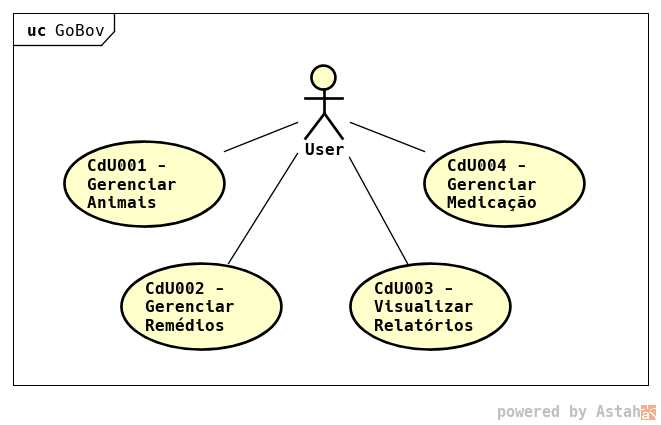
\includegraphics[width=6in]{../img/casosdeuso.png}

		Fonte: Autoria própria.
	\end{center}
\end{figure}

\subsection{PROTÓTIPOS DE TELA}

\begin{itemize}
\item IV001

Esta é a tela de login do sistema. Nela, o usuário pode se autenticar ou se registrar.
\begin{figure}[H]
	\begin{center}
		\caption{Login no sistema}
		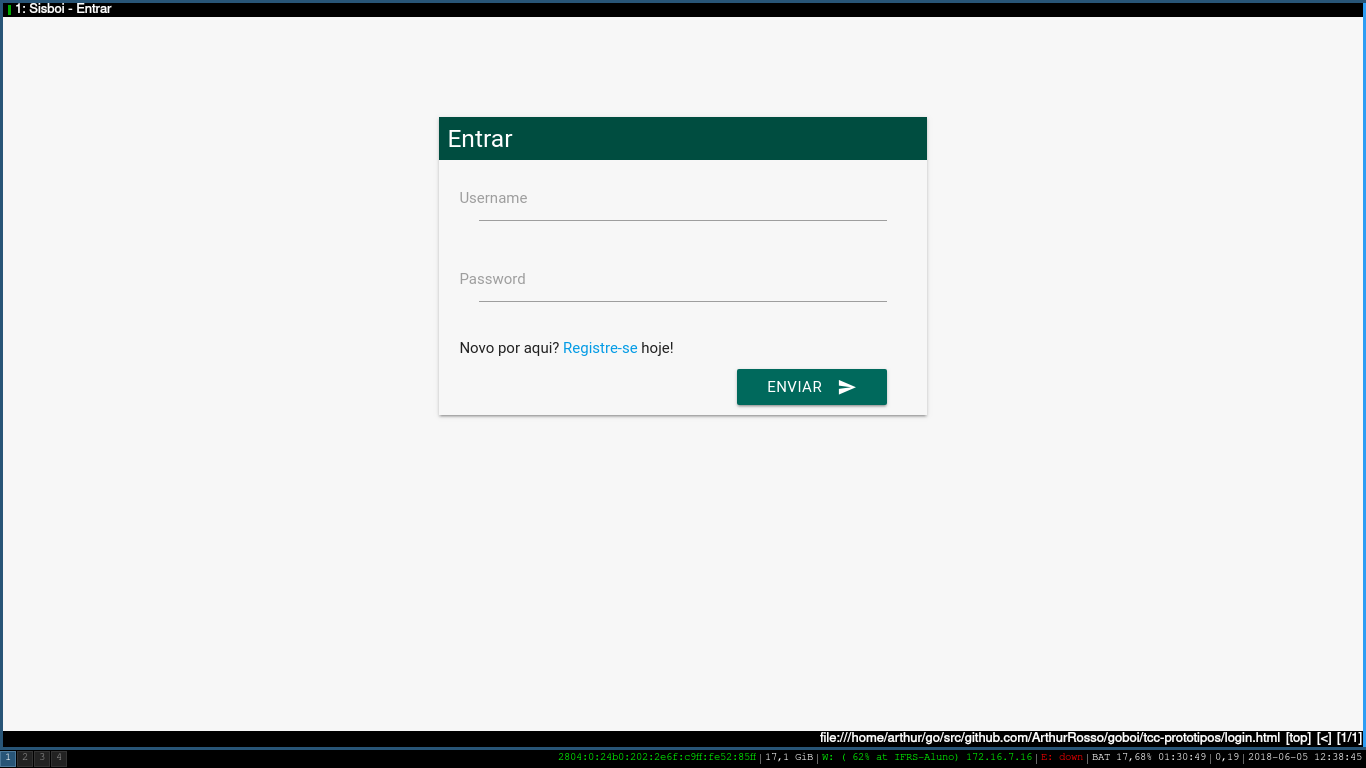
\includegraphics[width=13cm]{../img/prototipos/login.png}

		Fonte: Autoria própria.
	\end{center}
\end{figure}

\item IV002

A figura 5 é a tela inicial do sistema. Nela, o usuário pode acionar os casos de uso de gerenciar Animal, gerenciar Remédio, ou Gerenciar Medicações, também é possível ir direto para a página de algum animal, desde que já tenham feito algum manejo com ele.
\begin{figure}[H]
	\begin{center}
		\caption{Página inicial do sistema}
		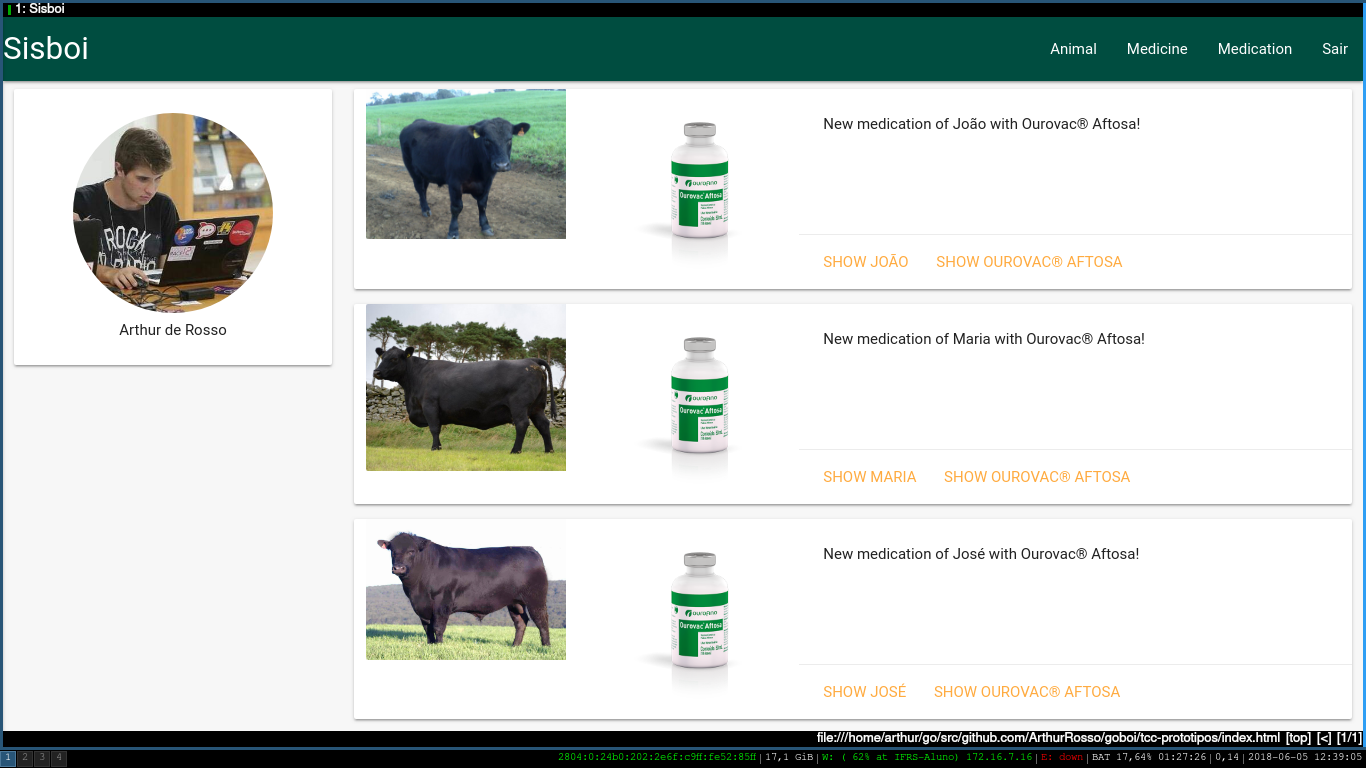
\includegraphics[width=13cm]{../img/prototipos/index.png}

		Fonte: Autoria própria.
	\end{center}
\end{figure}

\newpage
\item IV003

A figura 6 é a página do animal. Nela, o usuário pode adicionar um animal, deletar um animal ou ir para a tela de perfil do animal.
\begin{figure}[H]
	\begin{center}
		\caption{Página do animal}
		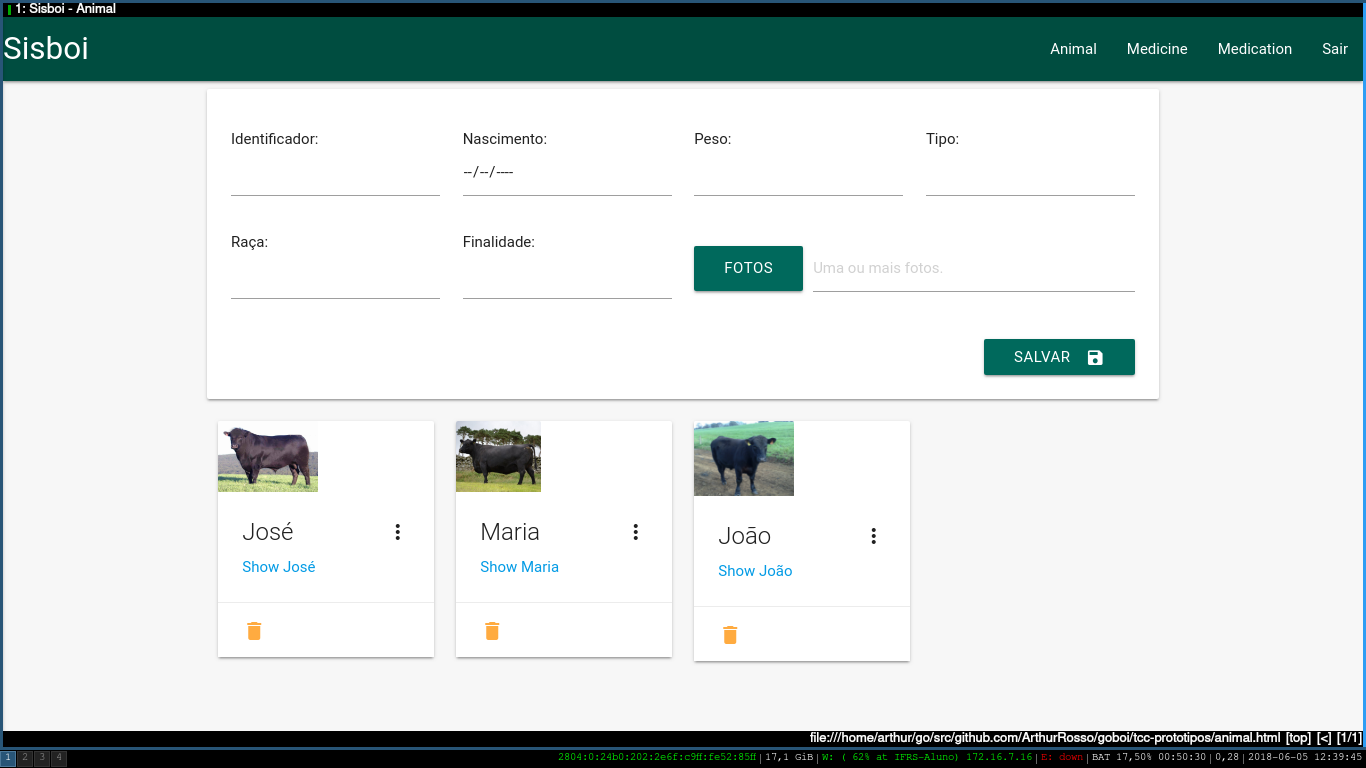
\includegraphics[width=13cm]{../img/prototipos/animal.png}

		Fonte: Autoria própria.
	\end{center}
\end{figure}

\item IV004

A figura 7 é a página do remédio. Nela, o usuário pode adicionar, deletar ou editar um remédio.
\begin{figure}[H]
	\begin{center}
		\caption{Página de remédios}
		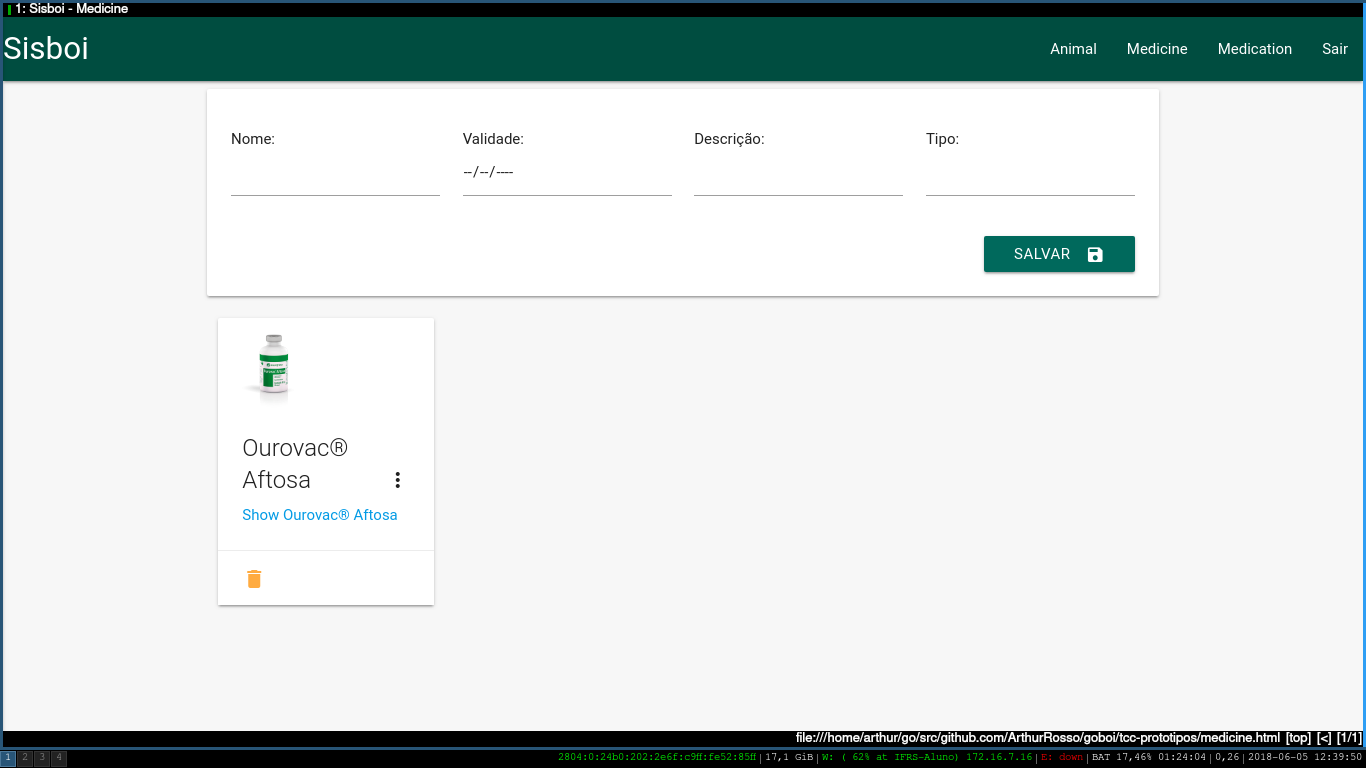
\includegraphics[width=13cm]{../img/prototipos/remedio.png}

		Fonte: Autoria própria.
	\end{center}
\end{figure}

\newpage
\item IV005

A figura 8 é a página da medicação. Nela, o usuário pode adicionar, deletar ou editar uma medicação.
\begin{figure}[H]
	\begin{center}
		\caption{Página de medicação}
		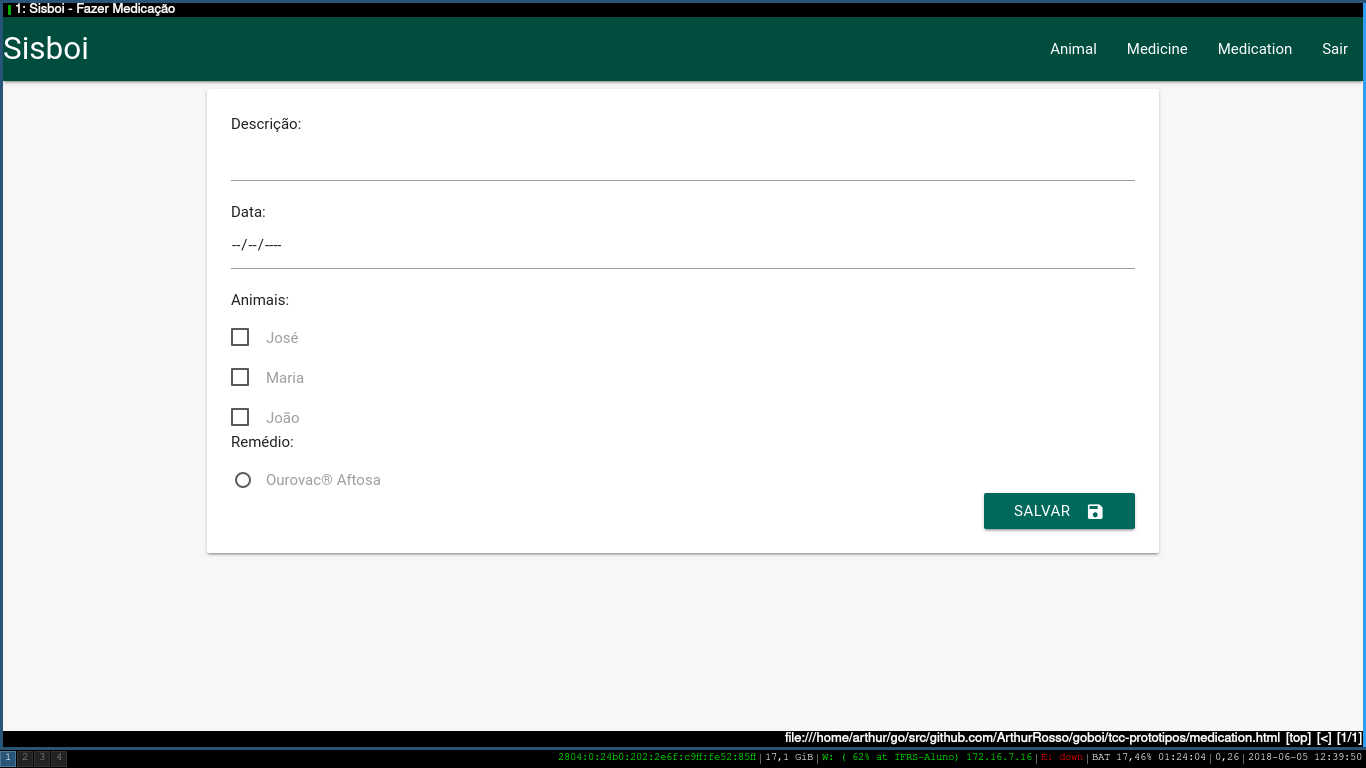
\includegraphics[width=13cm]{../img/prototipos/medicacao.png}

		Fonte: Autoria própria.
	\end{center}
\end{figure}

\item IV006

A figura 9 é a página de perfil do animal. Nela, o usuário pode editar, consultar detalhes ou gerenciar uma pesagem do animal.
\begin{figure}[H]
	\begin{center}
		\caption{Página de perfil do animal}
		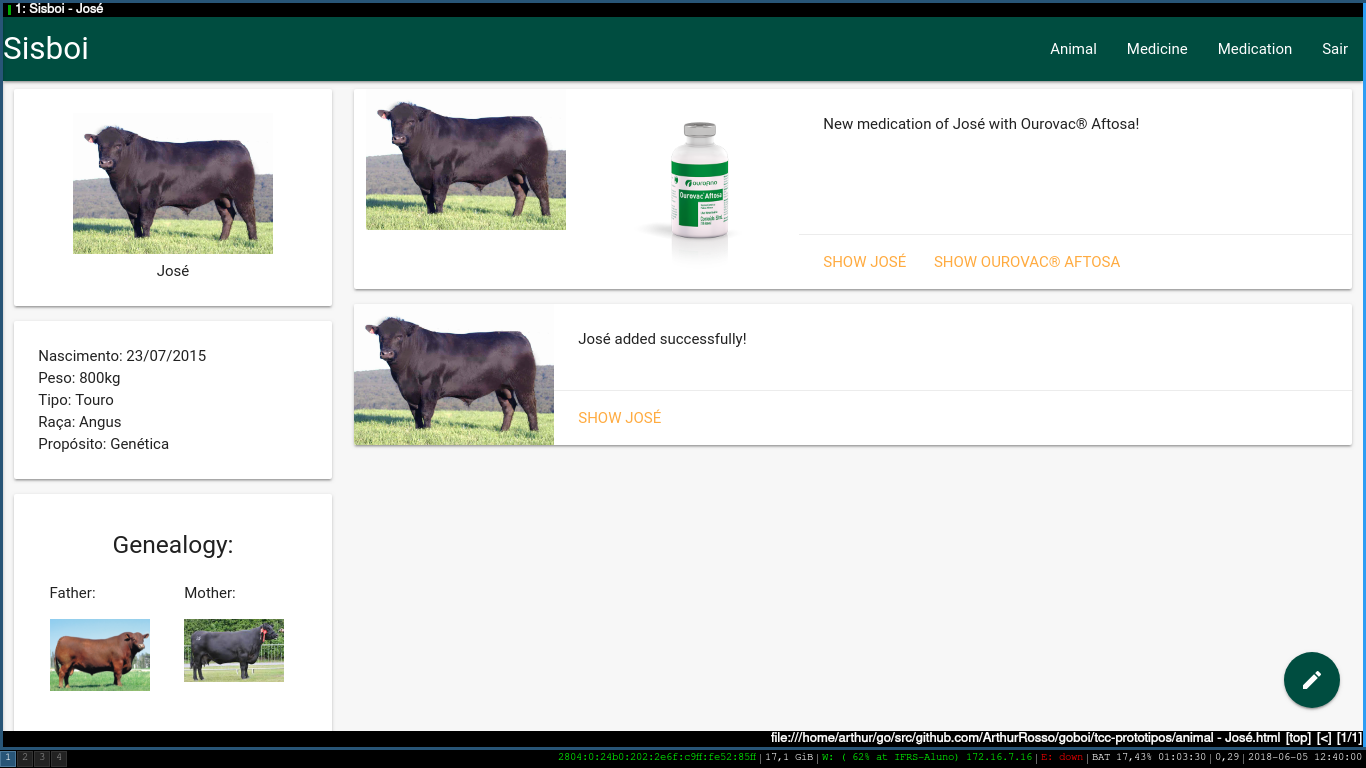
\includegraphics[width=13cm]{../img/prototipos/perfil.png}

		Fonte: Autoria própria.
	\end{center}
\end{figure}

\newpage
\item IV007

A figura 10 é a página de edição do animal. Nela o usuário pode editar as informações básicas do animal.
\begin{figure}[]
	\begin{center}
		\caption{Página de edição do animal}
		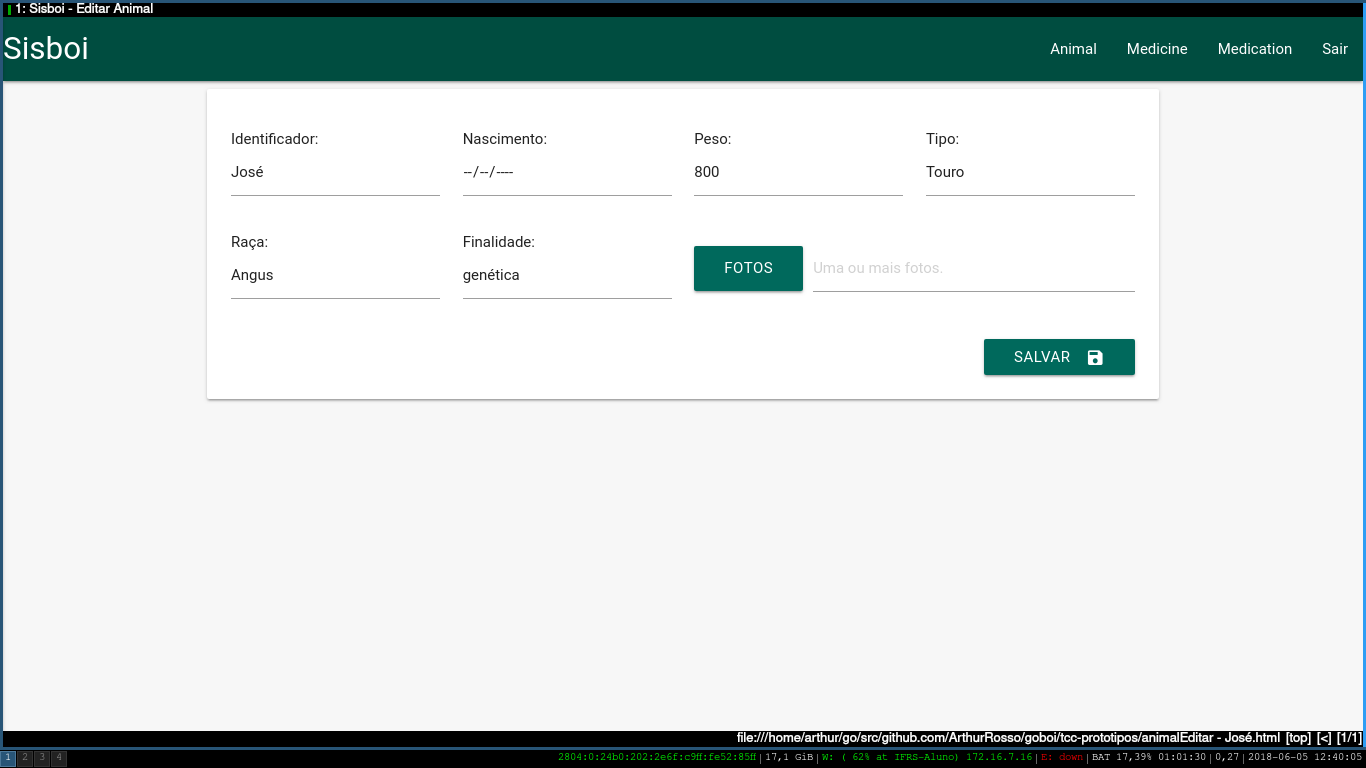
\includegraphics[width=13cm]{../img/prototipos/editar.png}

		Fonte: Autoria própria.
	\end{center}
\end{figure}

\item IV008

A figura 11 é a página de pesagem. Nela o usuário pode gerenciar o peso de um animal.
\begin{figure}[H]
	\begin{center}
		\caption{Página de pesagem do animal}
		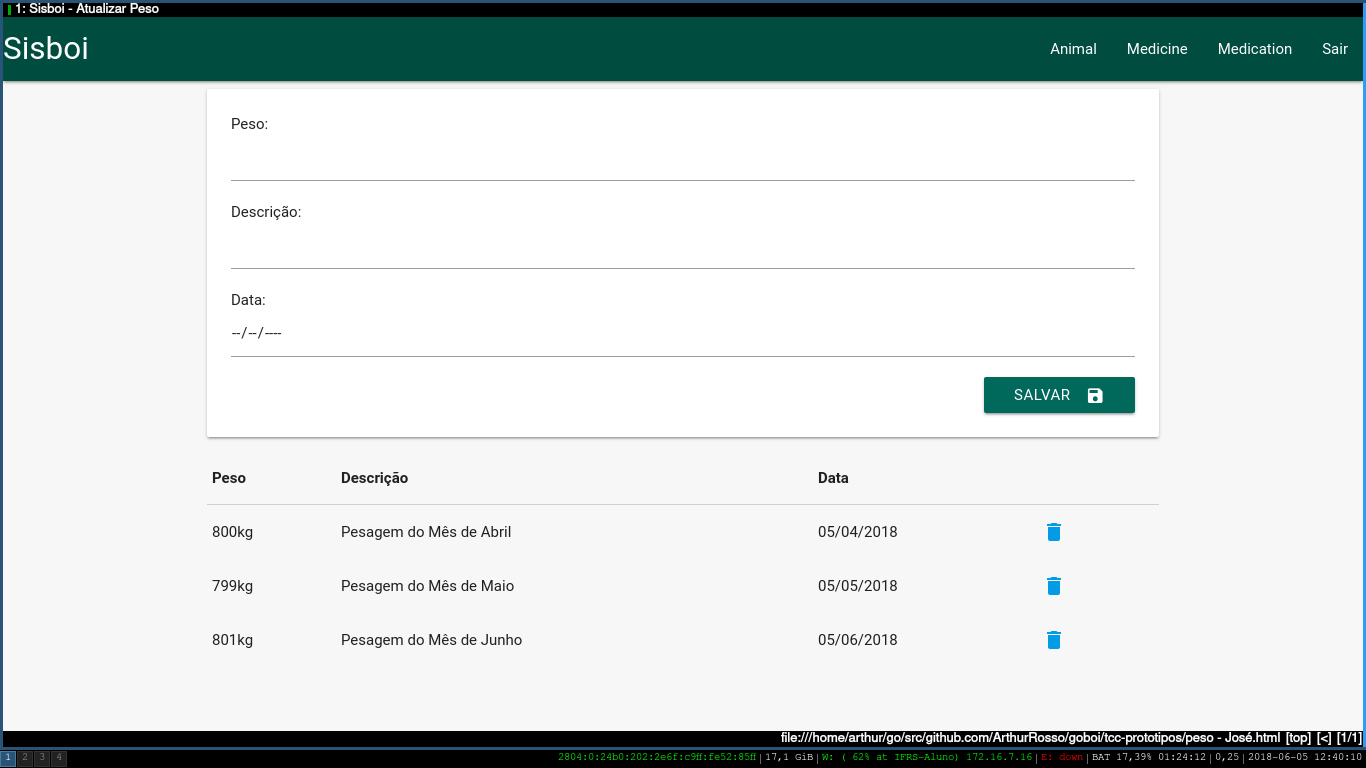
\includegraphics[width=13cm]{../img/prototipos/peso.png}

		Fonte: Autoria própria.
	\end{center}
\end{figure}

\end{itemize}
\subsection{OBJETIVO GERAL}
